\section{拒绝采样}
\label{sec:sgen-rejection}

前两节都要求目标分布有可以计算的分位数或可以抽样的分解。很多目标只给出一个密度公式，而且常常只知道到一个常数因子：$\pi(x)=\widetilde{p}(x)/Z$，其中$\widetilde{p}\ge0$可以逐点计算，归一化常数$Z=\int\widetilde{p}(x)\,\mathrm{d}x$却算不出来。模拟退火中的Gibbs分布$\exp(-f(x)/T)/Z_T$就是这样的目标（可参考\BookChapterRef{chap:random-search}{卷五第15章“随机搜索”}），状态多时$Z_T$是一个无法逐项求和的大和式。拒绝采样处理这类目标：从一个容易抽样的\term{建议分布}（proposal distribution）多抽一些候选，再按目标与建议的密度之比筛掉一部分。

这和用随机投点估计面积是同一个想法。在$\widetilde{p}$的图像下方均匀投点，点的横坐标就服从$\pi$；要在图像下方均匀投点，可以先在一个更大、容易投点的区域里均匀投点，再丢掉落在图像上方的点。

\subsection{接受规则的正确性}
\label{sec:sgen-rejection-correct}

设目标的未归一化密度$\widetilde{p}\ge0$满足$0<Z<\infty$；建议分布有密度$q$，可以直接抽样，密度可以计算；存在常数$M>0$，使
\begin{equation}
  \widetilde{p}(x)\le M\,q(x)\qquad\text{对一切}x\text{成立}.
  \label{eq:sgen-envelope}
\end{equation}
$Mq$称为包络，$M$称为\term{包络常数}（envelope constant）。式~\eqref{eq:sgen-envelope}蕴含：凡是$\widetilde{p}(x)>0$的地方都有$q(x)>0$，即建议分布覆盖了目标的全部质量所在。

\paragraph{一次试验}
抽候选$Y\sim q$，再抽与之独立的基础随机数$V$，当
\begin{equation}
  V\le\frac{\widetilde{p}(Y)}{M\,q(Y)}
  \label{eq:sgen-accept-rule}
\end{equation}
时接受$Y$，否则拒绝。$Y$落在$q(Y)=0$处的概率为零，比值总是有定义的；由式~\eqref{eq:sgen-envelope}，比值在$[0,1]$中，可以当作概率。几何上，点$(Y,\,V\,Mq(Y))$在包络$Mq$的图像下方均匀分布，接受规则就是“点落在$\widetilde{p}$的图像下方”。

\begin{theorem}[拒绝采样]
\label{thm:sgen-rejection}
在上述条件下，一次试验的接受概率是
\begin{equation}
  \mathbb{P}(\text{接受})=\frac{Z}{M},
  \label{eq:sgen-acceptance}
\end{equation}
给定接受时$Y$的条件分布是$\pi$。若独立重复试验直到第一次接受，记所用的试验次数为$N$、接受的候选为$X$，则$X\sim\pi$，$N\sim\operatorname{Geom}(Z/M)$，并且$X$与$N$独立。
\end{theorem}

\begin{proof}
对任意事件$A$，先对$Y$取条件，再对$Y$的密度积分。给定$Y=y$，接受的概率是$\widetilde{p}(y)/(Mq(y))$，因为$V$与$Y$独立。于是
\[
  \mathbb{P}(Y\in A,\ \text{接受})=\int_{A}q(y)\,\frac{\widetilde{p}(y)}{M\,q(y)}\,\mathrm{d}y=\frac{1}{M}\int_{A}\widetilde{p}(y)\,\mathrm{d}y=\frac{Z}{M}\,\pi(A).
\]
其中$q(y)=0$的点对积分没有贡献，由式~\eqref{eq:sgen-envelope}，那里$\widetilde{p}(y)=0$。取$A$为全空间，得到式~\eqref{eq:sgen-acceptance}。两式相除，$\mathbb{P}(Y\in A\mid\text{接受})=\pi(A)$。

记$a=Z/M$。各次试验使用互不重叠的基础随机数，相互独立。第$n$次才首次接受且接受的候选落在$A$中，意味着前$n-1$次都拒绝、第$n$次接受且候选在$A$中，所以
\[
  \mathbb{P}(N=n,\ X\in A)=(1-a)^{n-1}\cdot a\,\pi(A).
\]
对$A$取全空间得$\mathbb{P}(N=n)=(1-a)^{n-1}a$，即$N\sim\operatorname{Geom}(a)$；对$n$求和得$\mathbb{P}(X\in A)=\pi(A)$。联合概率等于两者之积，所以$X$与$N$独立。
\end{proof}

定理中各条件的作用如下。$0<Z<\infty$保证$\pi$是概率分布，也保证接受概率为正，否则会无限试下去。式~\eqref{eq:sgen-envelope}保证接受规则中的比值不超过$1$；它一旦失效，正确性随之失效，下面会看到后果。$V$与$Y$独立、各次试验独立，分别用在证明的第一步和第二步。整个算法只用到$\widetilde{p}$，不需要$Z$：$Z$的值只影响接受得多还是少，不影响接受下来的样本的分布。反过来，$M$必须真正满足式~\eqref{eq:sgen-envelope}，这是算法唯一需要预先保证的数。

\needspace{6\baselineskip}
\paragraph{变量}
\begin{itemize}
  \item $y$：当前候选，由建议分布生成。
  \item $v$：与候选配对的基础随机数，用于接受判定。
  \item $n$：已进行的试验次数。
\end{itemize}

\paragraph{初始化}
令$n=0$。下面用的例子是目标$\widetilde{p}(x)=x(1-x)$（$0\le x\le1$），建议分布$q=\operatorname{Unif}(0,1)$。$\widetilde{p}$在$x=1/2$处取最大值$1/4$，所以取$M=1/4$即满足式~\eqref{eq:sgen-envelope}。$Z=\int_0^1x(1-x)\,\mathrm{d}x=1/6$，归一化后$\pi(x)=6x(1-x)$是$\operatorname{Beta}(2,2)$的密度，但算法用不到这两个量。

\needspace{6\baselineskip}
\paragraph{每轮更新}
\begin{enumerate}
  \item \textbf{抽候选。}抽$y\sim q$与基础随机数$v$，令$n\leftarrow n+1$。例中第一轮用两个基础随机数$y=0.9$、$v=0.5$。
  \item \textbf{计算比值。}计算$r=\widetilde{p}(y)/(Mq(y))$。例中第一轮
  \[
    r=\frac{0.9\times0.1}{1/4}=0.36 .
  \]
  \item \textbf{判定。}若$v\le r$，接受$y$并停止；否则回到第1步。例中$0.5>0.36$，拒绝。第二轮取$y=0.37$、$v=0.80$，
  \[
    r=\frac{0.37\times0.63}{1/4}=0.9324\ge0.80,
  \]
  接受。
\end{enumerate}
最终得到样本$x=0.37$，用了$n=2$次试验、$4$个基础随机数。图~\ref{fig:sgen-rejection-envelope}(a)把这两次试验画成点$(y,\,vMq(y))$：$(0.9,0.125)$在抛物线上方，$(0.37,0.2)$在下方。

\begin{BookInlineFigure}
  \centering
  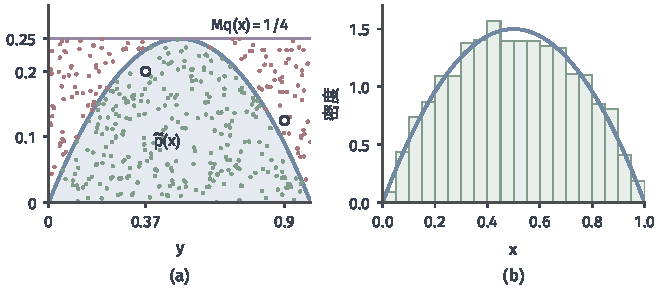
\includegraphics[width=112mm]{figures/07-probability/08-sampling-and-integration/matplotlib/sgen-rejection-envelope/figure.pdf}
  \caption{从$\operatorname{Unif}(0,1)$拒绝采样$\operatorname{Beta}(2,2)$，$\widetilde{p}(x)=x(1-x)$，$M=1/4$。(a)$400$个候选画成点$(y,\,vMq(y))$（种子$2$），紫线是包络$Mq=1/4$，蓝线下方浅蓝区域里的绿点被接受，上方的红点被拒绝；两个空心圆是正文中的两次试验。(b)$6000$个候选中被接受的点的直方图（接受比例$0.6625$），蓝线是$6x(1-x)$。}
  \label{fig:sgen-rejection-envelope}
\end{BookInlineFigure}

\paragraph{包络无效时}
若式~\eqref{eq:sgen-envelope}在某些点不成立，比值$\widetilde{p}/(Mq)$在那里超过$1$，判定$v\le r$必然通过，实际的接受概率是$\min\{1,\widetilde{p}/(Mq)\}$。把定理的第一步计算中的$\widetilde{p}/(Mq)$换成这个量，接受样本的密度正比于
\begin{equation}
  q(x)\min\Bigl\{1,\frac{\widetilde{p}(x)}{M\,q(x)}\Bigr\}=\frac{1}{M}\min\bigl\{\widetilde{p}(x),\,M\,q(x)\bigr\}.
  \label{eq:sgen-invalid-envelope}
\end{equation}
也就是说，目标在包络以上的部分被削平了。在上面的例子中错用$M=1/5$，$x(1-x)>1/5$的区间是$(0.276,0.724)$，输出的密度在这一段变成常数，中部的质量被系统地压低（图~\ref{fig:sgen-rejection-invalid}）。从直方图上看，偏差并不刺眼；程序也不会报错，因为每一步都“正常地”接受或拒绝。所以包络常数必须由推导保证，不能凭几次试算的最大比值来定。

\begin{BookInlineFigure}
  \centering
  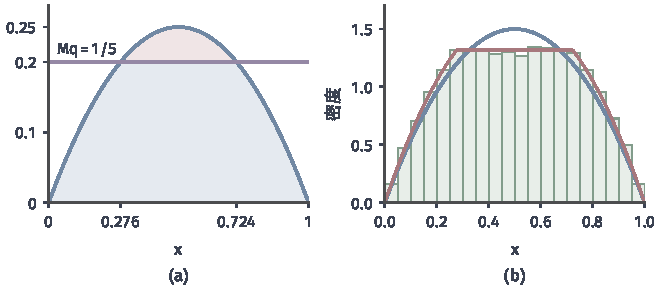
\includegraphics[width=112mm]{figures/07-probability/08-sampling-and-integration/matplotlib/sgen-rejection-invalid/figure.pdf}
  \caption{包络常数过小的后果。(a)蓝线是$\widetilde{p}(x)=x(1-x)$，紫线是错用的$Mq=1/5$，浅红区域是被削去的部分；(b)$20000$个候选中被接受点的直方图（种子$4$），红线是按式~\eqref{eq:sgen-invalid-envelope}归一化的输出密度，蓝线是目标$6x(1-x)$。}
  \label{fig:sgen-rejection-invalid}
\end{BookInlineFigure}

\subsection{接受率与生成成本}
\label{sec:sgen-rejection-cost}

拒绝采样总是正确的，问题在于要试多少次。由定理~\ref{thm:sgen-rejection}，试验次数$N$服从参数为$a=Z/M$的几何分布，于是得到一个样本平均所需的建议次数为
\begin{equation}
  \mathbb{E}[N]=\frac{M}{Z}.
  \label{eq:sgen-expected-trials}
\end{equation}
它就是包络下的面积$M$与目标下的面积$Z$之比，即投点区域中“浪费”的比例的倒数。例中$M/Z=(1/4)/(1/6)=1.5$，平均每个样本要试$1.5$次；图~\ref{fig:sgen-rejection-envelope}(b)中$6000$个候选的接受比例$0.6625$与理论值$2/3$相符。

若$\widetilde{p}=\pi$已经归一化，式~\eqref{eq:sgen-envelope}两边积分得$1\le M$，所以接受率$1/M$不超过$1$，等号当且仅当$q=\pi$（除去零概率集）。包络越贴近目标，$M$越接近$1$。

\paragraph{成本的组成}
一次试验的成本包括生成候选、计算$\widetilde{p}(y)$与$q(y)$、生成$v$。设一次试验的平均成本为$c$，得到$n$个样本的期望成本为$n\,c\,M/Z$，此外还有一次性的准备成本：求出有效的$M$。$M$最好取$\sup_x\widetilde{p}(x)/q(x)$，这需要解一个优化问题；取得太大虽然仍然正确，但成本按比例上升。两种成本的权衡在于：准备工作做一次，试验成本乘以样本数。

试验次数的波动也要计入。$N$的方差是$(1-a)/a^{2}$，接受率低时次数的分布有很长的右尾，生成固定个数的样本所需时间也随之波动。

\paragraph{高维中的接受率}
包络在高维中很难贴紧。设目标是$\mathcal{N}(\bm{0},\bm{I}_d)$，建议分布是$\mathcal{N}(\bm{0},\sigma^{2}\bm{I}_d)$，$\sigma>1$。两个归一化密度之比为
\[
  \frac{\pi(\bm{x})}{q(\bm{x})}=\sigma^{d}\exp\Bigl(-\frac{\lVert\bm{x}\rVert_2^{2}}{2}\bigl(1-\sigma^{-2}\bigr)\Bigr)\le\sigma^{d},
\]
等号在$\bm{x}=\bm{0}$处成立，所以最小的包络常数是$M=\sigma^{d}$，接受率为
\begin{equation}
  a=\sigma^{-d}.
  \label{eq:sgen-acceptance-dimension}
\end{equation}
每个坐标上建议分布只比目标宽一点，接受率也随维数指数下降。$\sigma=1.1$时，$d=10$的接受率约为$0.386$，$d=100$时约为$7.3\times10^{-5}$，平均每个样本要试一万多次。若$\sigma<1$，比值在$\lVert\bm{x}\rVert_2\to\infty$时趋于无穷，根本不存在包络：建议分布的尾部必须不比目标轻。

\begin{BookInlineFigure}
  \centering
  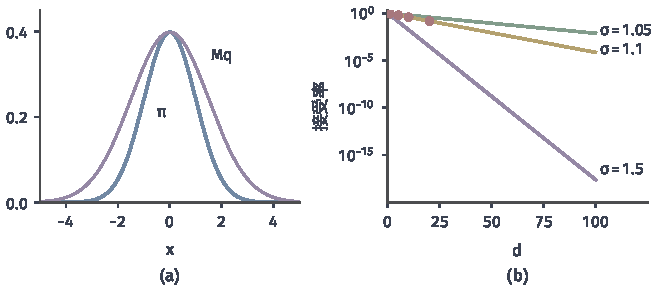
\includegraphics[width=112mm]{figures/07-probability/08-sampling-and-integration/matplotlib/sgen-rejection-dimension/figure.pdf}
  \caption{高斯目标、高斯建议时的拒绝采样。(a)$d=1$、$\sigma=1.5$，蓝线是目标$\pi$，紫线是包络$Mq$，二者只在$x=0$处相切；(b)接受率$\sigma^{-d}$随维数$d$的变化（对数纵轴），绿、黄、紫依次为$\sigma=1.05,1.1,1.5$，红点是$\sigma=1.1$、$d=1,5,10,20$时各$20$万个候选的模拟接受比例（种子$8$）。}
  \label{fig:sgen-rejection-dimension}
\end{BookInlineFigure}

图~\ref{fig:sgen-rejection-dimension}(a)说明了原因：包络只在一点与目标相切，其余地方都留有空隙，空隙所占的比例按维数相乘。一维时浪费不到一半，一百维时几乎全部浪费。拒绝采样在低维、能找到贴身包络的问题中很有效，在高维中通常只作为其他方法的一个组成部分。对那些连有效包络都写不出来的高维目标，需要换一种思路，这就是下一节的链式更新。
